\section{Discriminant Performance}

The matrix element analysis computes two quantites for each event,
$D_{s}(\vec{x})$ and $D_{t}(\vec{x})$, which are the discriminants for $s$-channel
and $t$-channel, respectively. This section shows several performance curves for
for signal and background Monte Carlo events. Each curve has been normalized to
unit area in order to show differences in shapes for the signal and background.

\subsection{$s$-channel Performance}

\vspace{0.1in}
\begin{figure}[!h!tbp]
\begin{center}
\subfigure[]{
	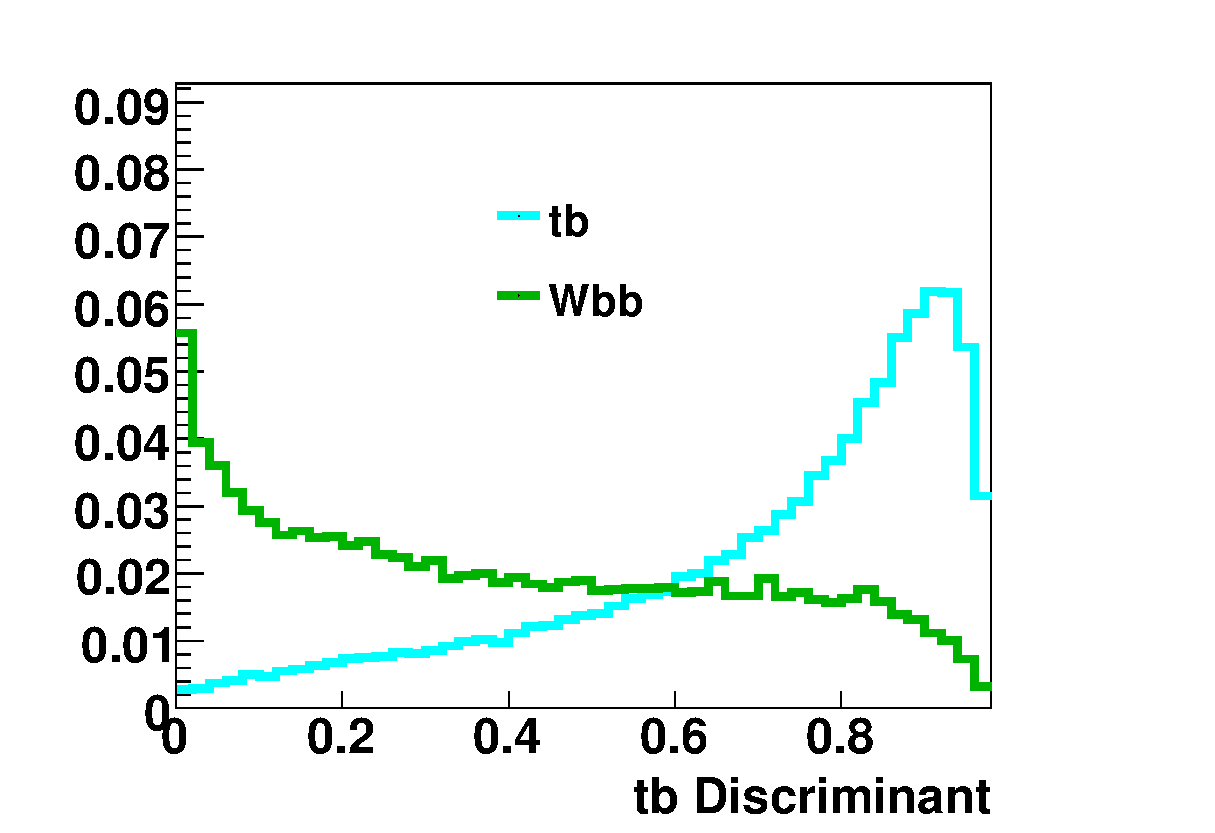
\includegraphics[width=0.48\textwidth]{figures/performance/tb_Discriminant__schannel_wbb.eps}
}
\subfigure[]{
	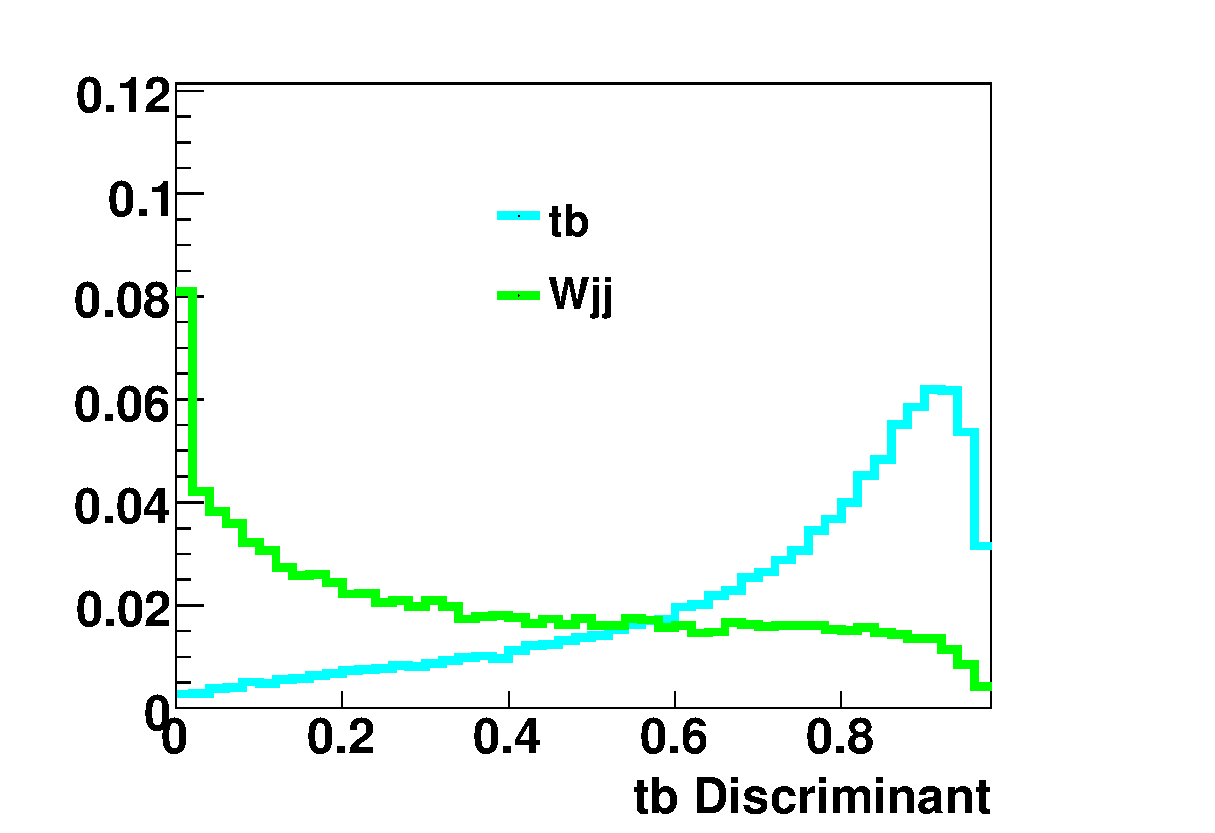
\includegraphics[width=0.48\textwidth]{figures/performance/tb_Discriminant__schannel_wjj.eps}
}
\subfigure[]{
	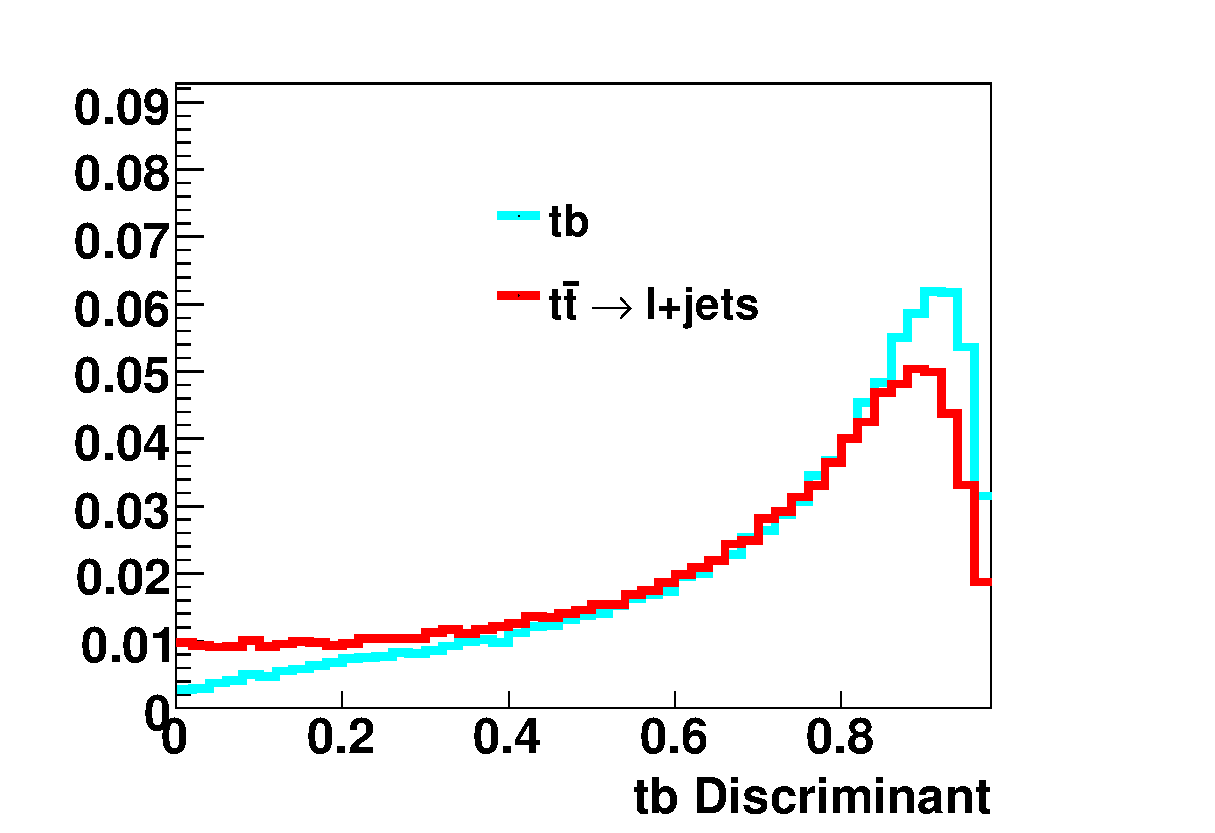
\includegraphics[width=0.48\textwidth]{figures/performance/tb_Discriminant__schannel_lepjets.eps}
}
\subfigure[]{
	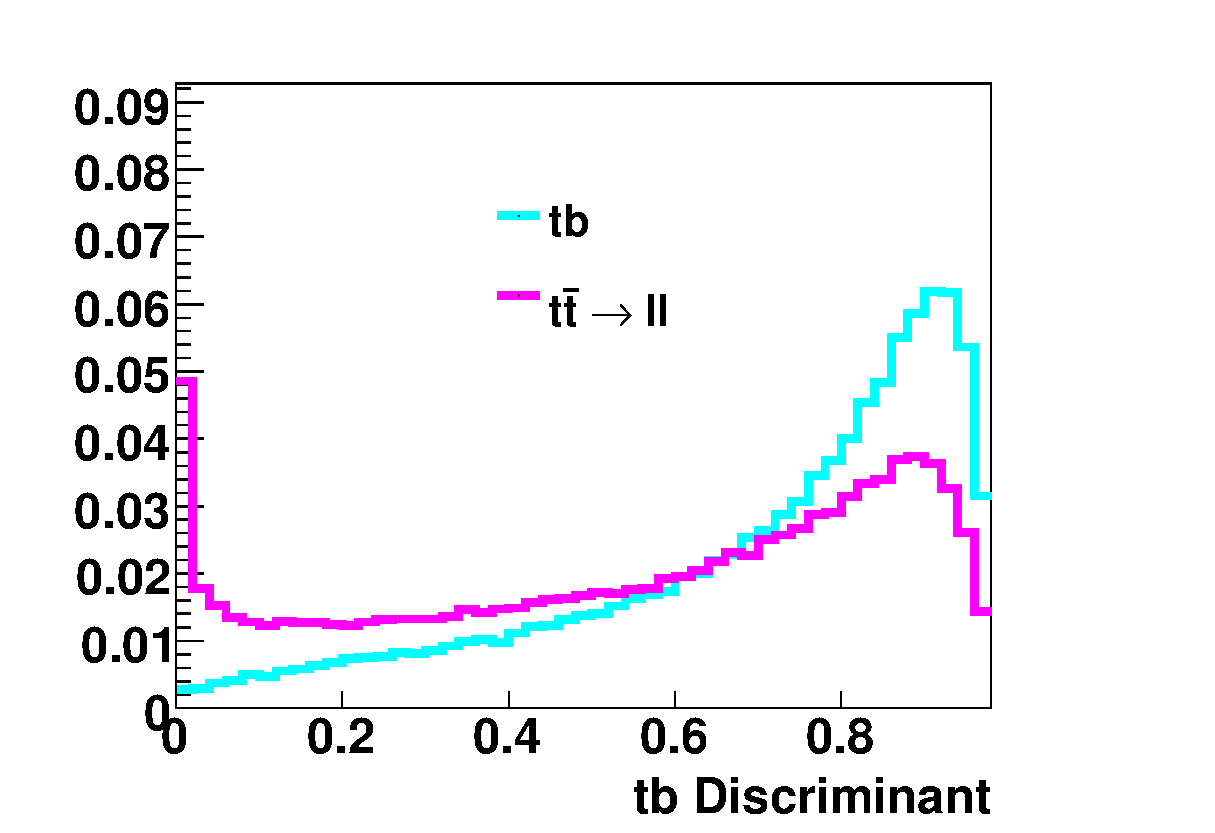
\includegraphics[width=0.48\textwidth]{figures/performance/tb_Discriminant__schannel_dilepton.eps}
}
\end{center}
\vspace{-0.1in}
\caption{Discriminant performance for $s$-channel (cyan) against (a) Wbb (green),
(b) Wjj (light green), (c) \lepjets (red), and (d) \dilepton (pink)}
\end{figure}


\clearpage
\subsection{$t$-channel Performance}

\vspace{0.1in}
\begin{figure}[!h!tbp]
\begin{center}
\subfigure[]{
	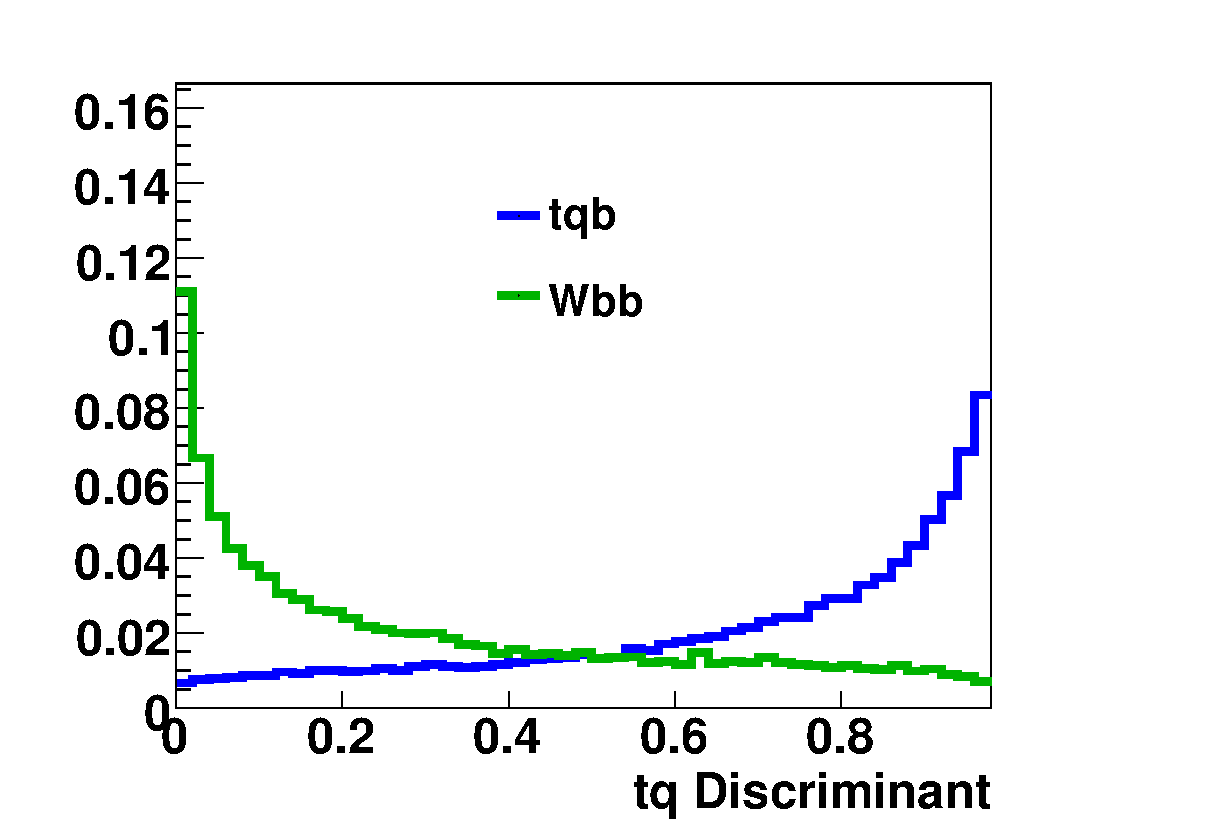
\includegraphics[width=0.48\textwidth]{figures/performance/tq_Discriminant__tchannel_wbb.eps}
}
\subfigure[]{
	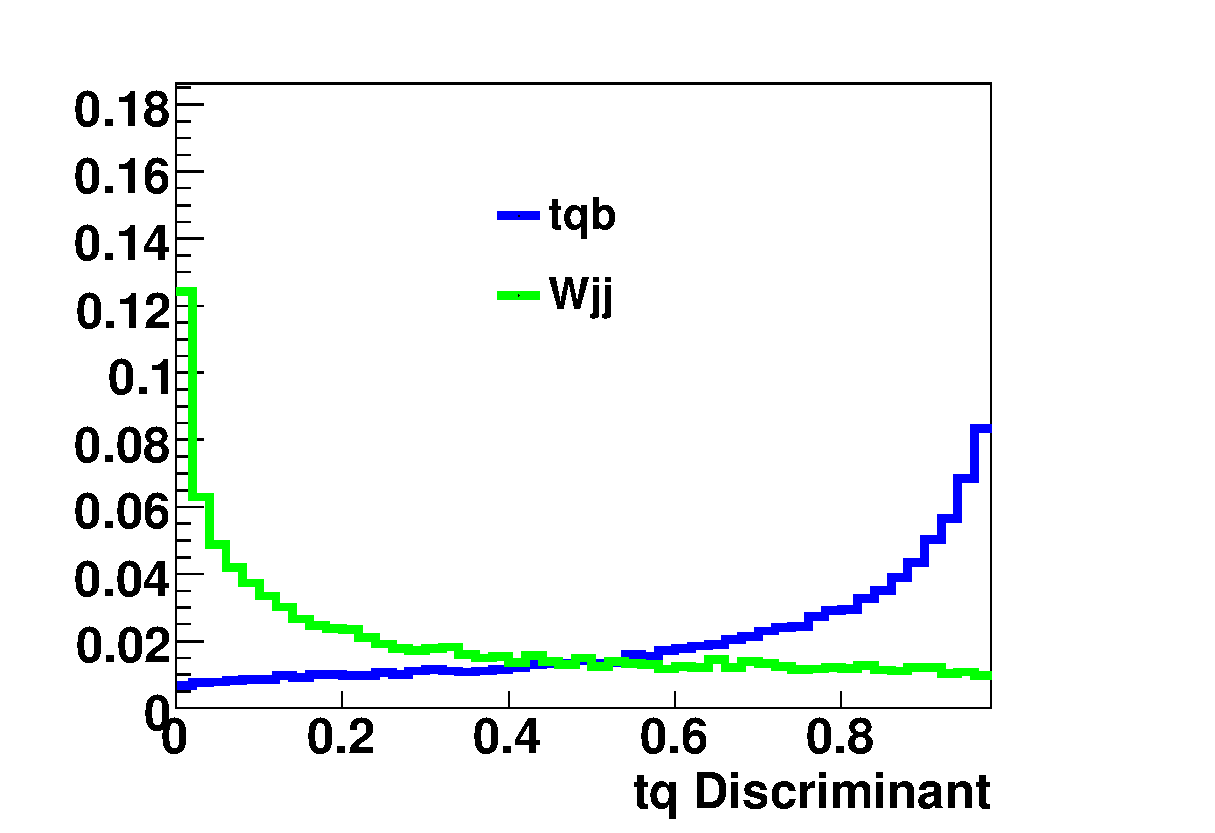
\includegraphics[width=0.48\textwidth]{figures/performance/tq_Discriminant__tchannel_wjj.eps}
}
\subfigure[]{
	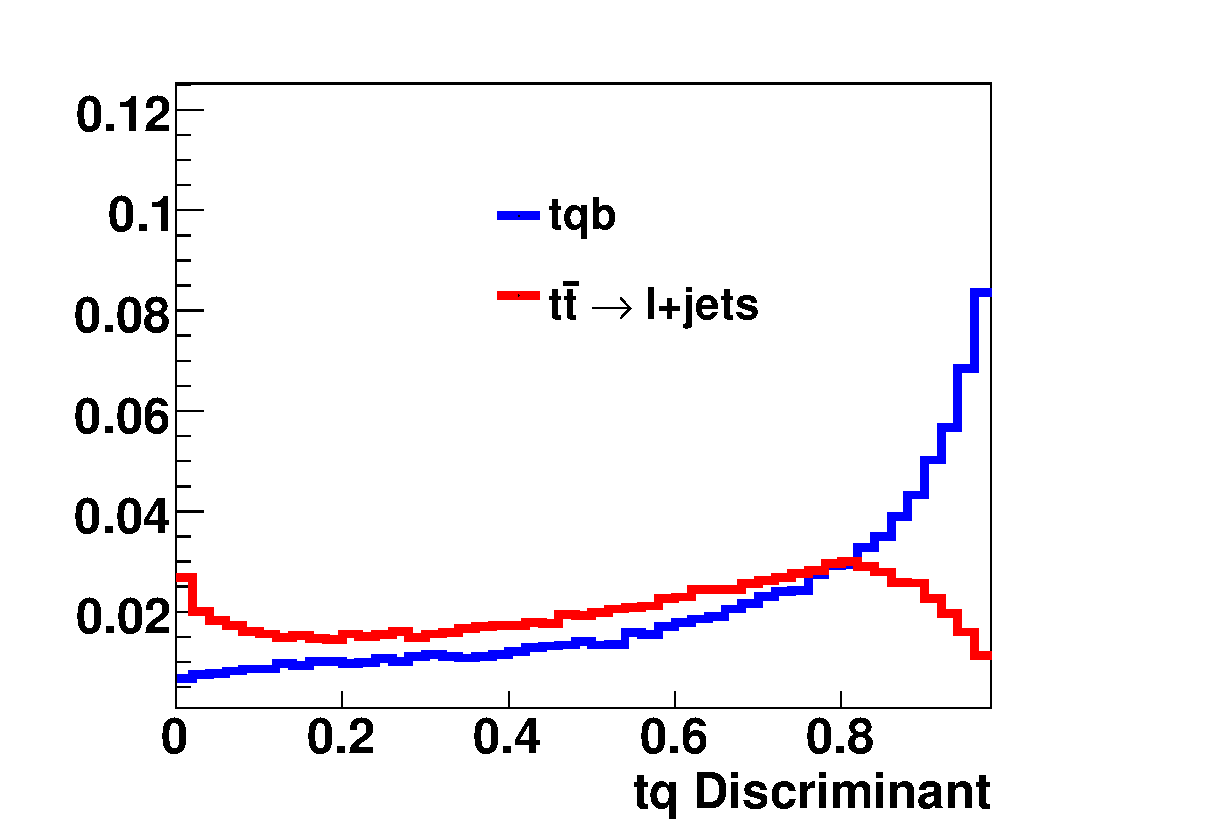
\includegraphics[width=0.48\textwidth]{figures/performance/tq_Discriminant__tchannel_lepjets.eps}
}
\subfigure[]{
	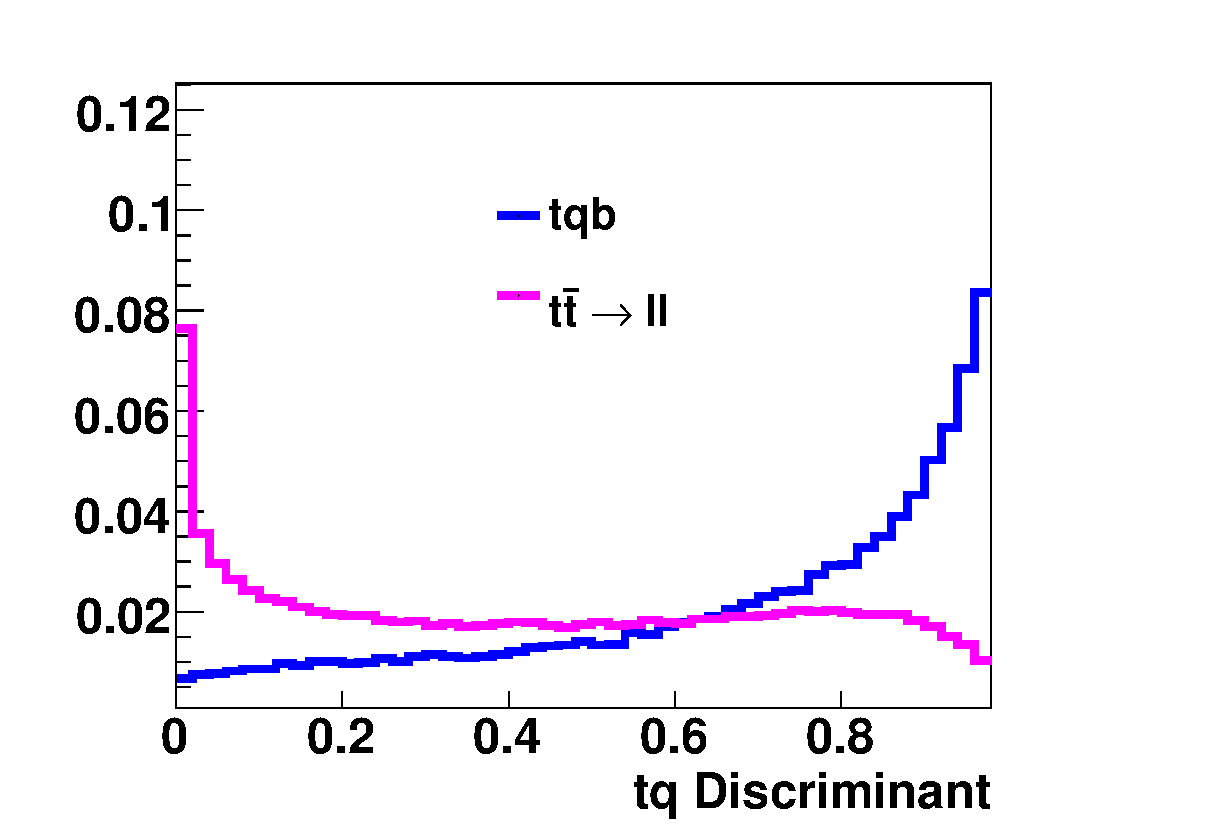
\includegraphics[width=0.48\textwidth]{figures/performance/tq_Discriminant__tchannel_dilepton.eps}
}
\end{center}
\vspace{-0.1in}
\caption{Discriminant performance for $t$-channel (blue) against (a) Wbb (green),
(b) Wjj (light green), (c) \lepjets (red), and (d) \dilepton (pink)}
\end{figure}

